\documentclass[journal,12pt,twocolumn]{IEEEtran}

\usepackage{cite}
\usepackage{amsmath,amssymb,amsfonts,amsthm}
\usepackage{algorithmic}
\usepackage{graphicx}
\usepackage{textcomp}
\usepackage{xcolor}
\usepackage{txfonts}
\usepackage{listings}
\usepackage{enumitem}
\usepackage{mathtools}
\usepackage{gensymb}
\usepackage[breaklinks=true]{hyperref}
\usepackage{tkz-euclide} % loads TikZ and tkz-base
\usepackage{circuitikz}

\newtheorem{theorem}{Theorem}[section]
\newtheorem{problem}{Problem}
\newtheorem{proposition}{Proposition}[section]
\newtheorem{lemma}{Lemma}[section]
\newtheorem{corollary}[theorem]{Corollary}
\newtheorem{example}{Example}[section]
\newtheorem{definition}[problem]{Definition}
\newcommand{\BEQA}{\begin{eqnarray}}
\newcommand{\EEQA}{\end{eqnarray}}
\newcommand{\define}{\stackrel{\triangle}{=}}
\newcommand\figref{Fig.~\ref}
\newcommand\tabref{Table~\ref}

\lstset{
    frame=single,
    breaklines=true,
    columns=fullflexible
}

\providecommand{\mbf}{\mathbf}
\providecommand{\pr}[1]{\ensuremath{\Pr\left(#1\right)}}
\providecommand{\qfunc}[1]{\ensuremath{Q\left(#1\right)}}
\providecommand{\sbrak}[1]{\ensuremath{{}\left[#1\right]}}
\providecommand{\lsbrak}[1]{\ensuremath{{}\left[#1\right.}}
\providecommand{\rsbrak}[1]{\ensuremath{{}\left.#1\right]}}
\providecommand{\brak}[1]{\ensuremath{\left(#1\right)}}
\providecommand{\lbrak}[1]{\ensuremath{\left(#1\right.}}
\providecommand{\rbrak}[1]{\ensuremath{\left.#1\right)}}
\providecommand{\cbrak}[1]{\ensuremath{\left\{#1\right\}}}
\providecommand{\lcbrak}[1]{\ensuremath{\left\{#1\right.}}
\providecommand{\rcbrak}[1]{\ensuremath{\left.#1\right\}}}
\theoremstyle{remark}
\newtheorem{rem}{Remark}
\newcommand{\sgn}{\mathop{\mathrm{sgn}}}
\providecommand{\abs}[1]{\left\vert#1\right\vert}
\providecommand{\res}[1]{\Res\displaylimits_{#1}}
\providecommand{\norm}[1]{\left\lVert#1\right\rVert}
\providecommand{\mtx}[1]{\mathbf{#1}}
\providecommand{\mean}[1]{E\left[ #1 \right]}
\providecommand{\fourier}{\overset{\mathcal{F}}{ \rightleftharpoons}}
\providecommand{\system}{\overset{\mathcal{H}}{ \longleftrightarrow}}
\newcommand{\solution}{\noindent \textbf{Solution: }}
\newcommand{\cosec}{\,\text{cosec}\,}
\providecommand{\dec}[2]{\ensuremath{\overset{#1}{\underset{#2}{\gtrless}}}}
\newcommand{\myvec}[1]{\ensuremath{\begin{pmatrix}#1\end{pmatrix}}}
\newcommand{\mydet}[1]{\ensuremath{\begin{vmatrix}#1\end{vmatrix}}}
\renewcommand{\abstractname}{Question}

\let\vec\mathbf

\newcommand{\permcomb}[4][0mu]{{{}^{#3}\mkern#1#2_{#4}}}
\newcommand{\comb}[1][-1mu]{\permcomb[#1]{C}}

\newcommand \tab [1][1cm]{\hspace*{#1}}

\title{NCERT Discrete 11.5.9.2}
\author{EE23BTECH11201 - ABBURI TANUSHA}

\begin{document}
\maketitle
\textbf{Question:} 
The sum of three numbers in an arithmetic progression (AP) is $24$ and the product of those three numbers is $440$, find the values of the three numbers.

\solution
The following information is provided in the question:
\begin{table}[h]
 	\centering
 	\resizebox{6 cm}{!}{
 		

    \begin{tabular}{|c|c|c|}
        \hline
        \textbf{Parameter} & \textbf{Value} & \textbf{Description} \\
        \hline
        a     & 8 & First term \\
        d     & 5 & common difference\\
        xi(0) & 8 & First term \\
        \hline
    \end{tabular}
    
    



 	}
 	\vspace{6 pt}
 	\caption{Parameters}
 	\label{tab:my_label} 
 \end{table}
\newline
Let the three numbers in the arithmetic progression be denoted as $a - d$, $a$, and $a + d$. Then,
\begin{align}
    \brak{a-d} + a + \brak{a + d} &= 3a \\
     3a &= 24 \\
    a &= 8 \\
    \label{eq:eq3} 
    \brak{a - d} \times a \times \brak{a + d} &= 440 \\
  From \eqref{eq:eq3} :
    \brak{8} \times \brak{8-d} \times \brak{8+d} &= 440 \\
    \brak{8-d} \times \brak{8+d} &= 55 \\
    d &= 3 \\
    x(n) &= \brak{x(0) + n \times d} u(n) \\
    x(n) &= \brak{2 + 3n}u(n)\\
    X(z) &= \frac{5 - 8z^{-1}}{(1-z^{-1})^2} ; |Z|>1
\end{align}
Therefore, The required three numbers in AP is 5,8 and 11.

\begin{figure}[h!]
  \centering
  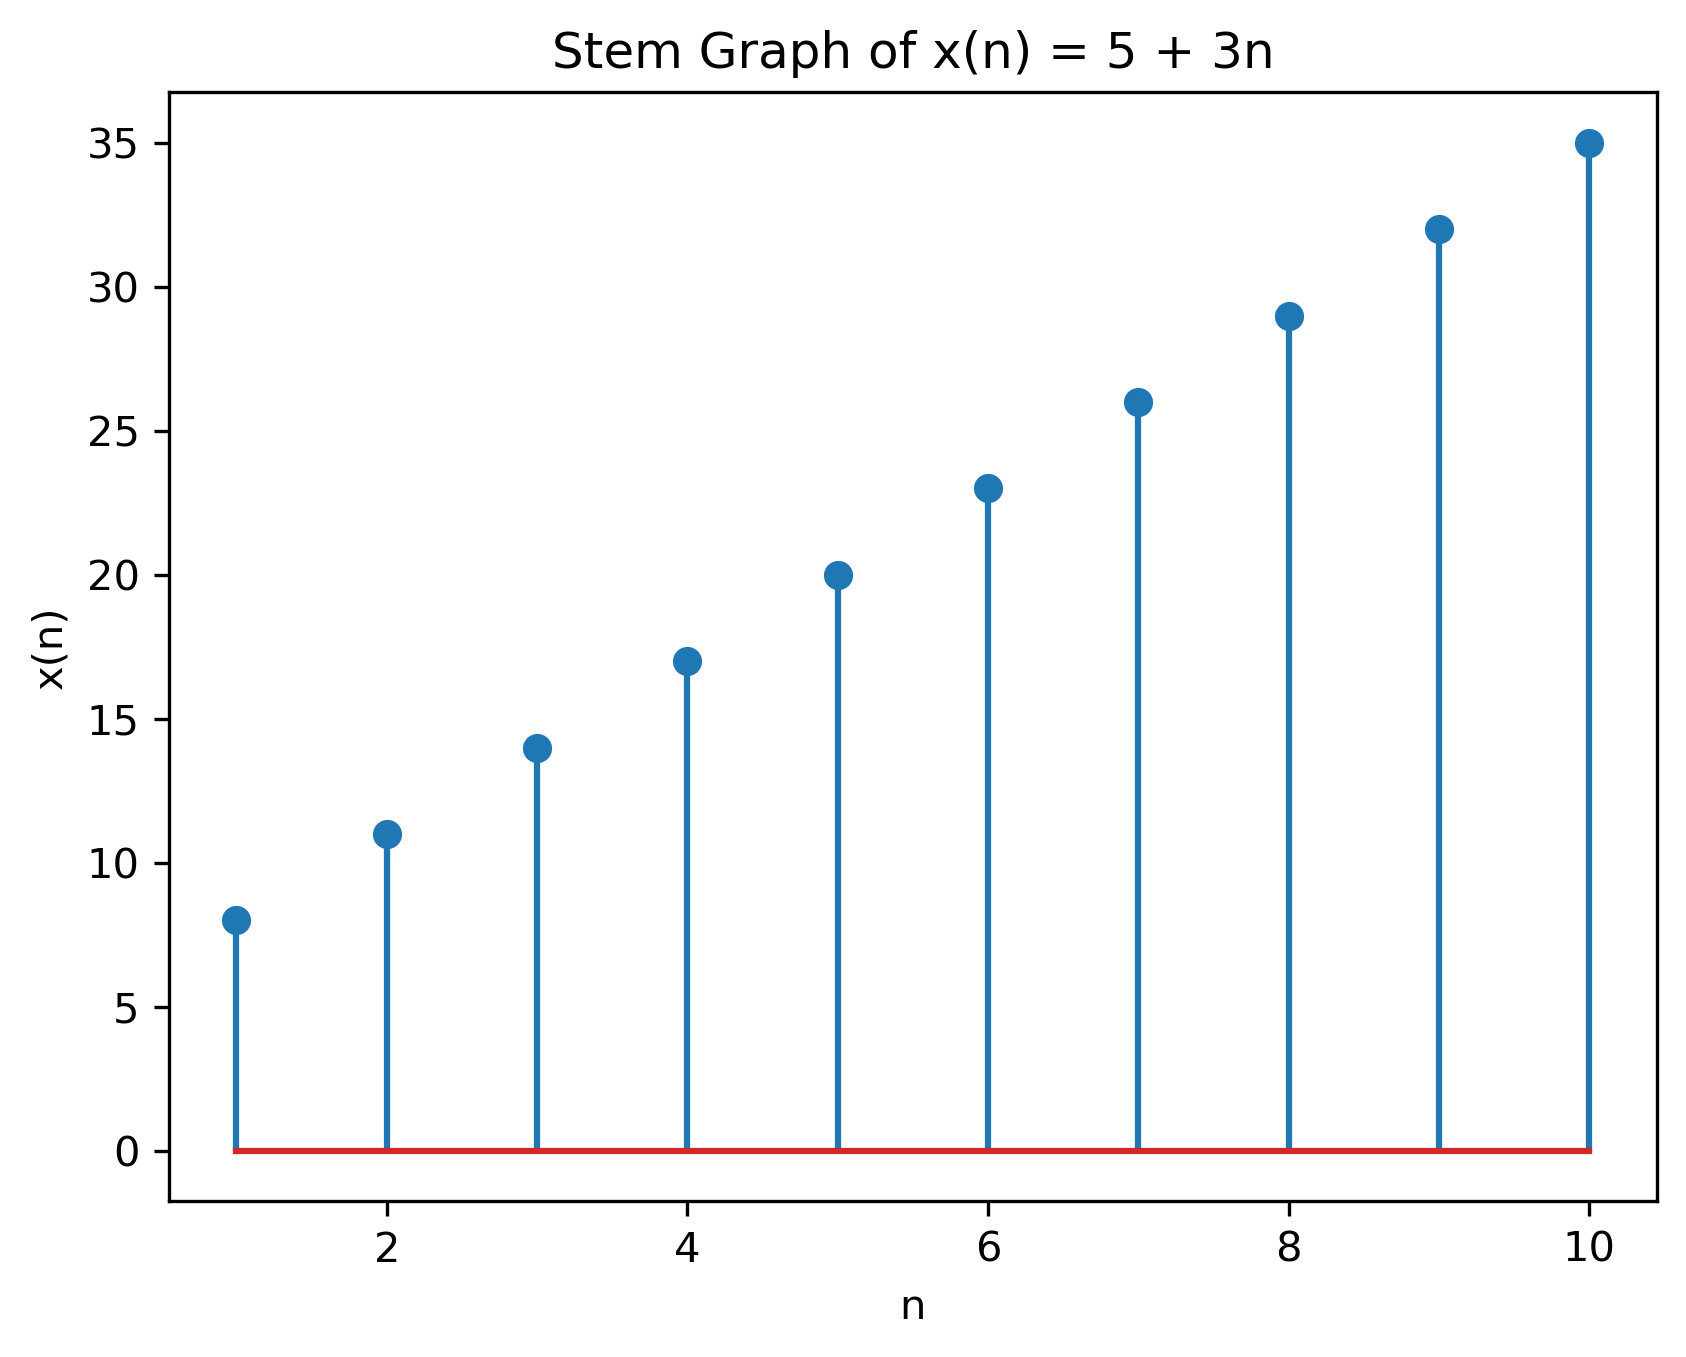
\includegraphics[width=0.3\textwidth]{figs/tan_plot.png} 
  \caption{stem plots of $x(n)$ }
  \label{fig:1}
\end{figure}
\end{document}

